% Options for packages loaded elsewhere
\PassOptionsToPackage{unicode}{hyperref}
\PassOptionsToPackage{hyphens}{url}
%
\documentclass[
  12pt,
]{article}
\title{Harmful Algal Blooms in Southern California}
\usepackage{etoolbox}
\makeatletter
\providecommand{\subtitle}[1]{% add subtitle to \maketitle
  \apptocmd{\@title}{\par {\large #1 \par}}{}{}
}
\makeatother
\subtitle{\url{https://github.com/curtx562/Cha_OBrien_ENV872_EDA_FinalProject}}
\author{Curtis Cha \& Bryce O'Brien}
\date{}

\usepackage{amsmath,amssymb}
\usepackage{lmodern}
\usepackage{iftex}
\ifPDFTeX
  \usepackage[T1]{fontenc}
  \usepackage[utf8]{inputenc}
  \usepackage{textcomp} % provide euro and other symbols
\else % if luatex or xetex
  \usepackage{unicode-math}
  \defaultfontfeatures{Scale=MatchLowercase}
  \defaultfontfeatures[\rmfamily]{Ligatures=TeX,Scale=1}
  \setmainfont[]{Times New Roman}
\fi
% Use upquote if available, for straight quotes in verbatim environments
\IfFileExists{upquote.sty}{\usepackage{upquote}}{}
\IfFileExists{microtype.sty}{% use microtype if available
  \usepackage[]{microtype}
  \UseMicrotypeSet[protrusion]{basicmath} % disable protrusion for tt fonts
}{}
\makeatletter
\@ifundefined{KOMAClassName}{% if non-KOMA class
  \IfFileExists{parskip.sty}{%
    \usepackage{parskip}
  }{% else
    \setlength{\parindent}{0pt}
    \setlength{\parskip}{6pt plus 2pt minus 1pt}}
}{% if KOMA class
  \KOMAoptions{parskip=half}}
\makeatother
\usepackage{xcolor}
\IfFileExists{xurl.sty}{\usepackage{xurl}}{} % add URL line breaks if available
\IfFileExists{bookmark.sty}{\usepackage{bookmark}}{\usepackage{hyperref}}
\hypersetup{
  pdftitle={Harmful Algal Blooms in Southern California},
  pdfauthor={Curtis Cha \& Bryce O'Brien},
  hidelinks,
  pdfcreator={LaTeX via pandoc}}
\urlstyle{same} % disable monospaced font for URLs
\usepackage[margin = 2.54cm]{geometry}
\usepackage{graphicx}
\makeatletter
\def\maxwidth{\ifdim\Gin@nat@width>\linewidth\linewidth\else\Gin@nat@width\fi}
\def\maxheight{\ifdim\Gin@nat@height>\textheight\textheight\else\Gin@nat@height\fi}
\makeatother
% Scale images if necessary, so that they will not overflow the page
% margins by default, and it is still possible to overwrite the defaults
% using explicit options in \includegraphics[width, height, ...]{}
\setkeys{Gin}{width=\maxwidth,height=\maxheight,keepaspectratio}
% Set default figure placement to htbp
\makeatletter
\def\fps@figure{htbp}
\makeatother
\setlength{\emergencystretch}{3em} % prevent overfull lines
\providecommand{\tightlist}{%
  \setlength{\itemsep}{0pt}\setlength{\parskip}{0pt}}
\setcounter{secnumdepth}{5}
\usepackage{booktabs}
\usepackage{longtable}
\usepackage{array}
\usepackage{multirow}
\usepackage{wrapfig}
\usepackage{float}
\usepackage{colortbl}
\usepackage{pdflscape}
\usepackage{tabu}
\usepackage{threeparttable}
\usepackage{threeparttablex}
\usepackage[normalem]{ulem}
\usepackage{makecell}
\usepackage{xcolor}
\ifLuaTeX
  \usepackage{selnolig}  % disable illegal ligatures
\fi

\begin{document}
\maketitle

\newpage
\tableofcontents
\newpage
\listoftables 
\newpage
\listoffigures
\newpage

\begin{center}\rule{0.5\linewidth}{0.5pt}\end{center}

\hypertarget{rationale-and-research-questions}{%
\section{Rationale and Research
Questions}\label{rationale-and-research-questions}}

Harmful Algal Blooms (HABs) threaten marine resources, coastal economies
and human health globally. These phenomena, characterized by the rapid
growth followed by the rapid decay of aquatic cyanobacteria, are
responsible for the death of marine mammals and birds, the intoxication
of fish and shellfish and serious health implications in human
populations (Moore et al.~2008).

In the context of North America's Pacific coast, HAB events are
typically caused by marine diatoms or dinoflagellates (Lewitus et
al.~2012). One example of a harmful marine diatom is Pseudo-nitzschia;
this genus is responsible for a significant portion of Harmful Algal
Bloom events in coastal California (Zhu et al.~2017). Although some
species of Pseudo-nitzschia are nontoxigenic, many produce a neurotoxin
called domoic acid (DA) which is known to cause death in marine mammals
and birds. DA is also the cause of amnesic shellfish poisoning in
humans, as this toxin bioaccumulates in fish and shellfish (Smith et
al.~2017).

A second dominant harmful algal genus in coastal California is
Alexandrium, which is a dinoflagellate known to produce toxins
responsible for paralytic shellfish poisoning (Trainer et al.~2020). It
is important to note that blooms of these two genera are defined by
unique threshold concentrations: according to the Southern California
Coastal Ocean Observing System as well as the Woods Hole Oceanographic
Institution's Outfall Monitoring Science Advisory Panel, a
Pseudo-nitzschia bloom is defined as an event of over 10,000 cells/liter
whereas an Alexandrium bloom is defined as an event of over 100
cells/liter.

In this project, we utilized time series analyses and linear regression
models to explore: 1) how concentrations of Pseudo-nitzschia and
Alexandrium change over time and 2) which environmental variables
(chemical, geographical, and physical factors) help describe variation
in these concentrations. We narrowed our project scope to focus on the
five following locations in southern California: San Luis Obsipo, Santa
Barbara, Santa Monica, Newport and San Diego. Findings from this study
are important in that they better our understanding of how harmful algal
blooms are changing in prevalence or distribution thoughout southern
California and which environmental factors are driving these changes.

\newpage

\hypertarget{dataset-information}{%
\section{Dataset Information}\label{dataset-information}}

Data for this project is sourced from the regional HAB monitoring system
of Southern California, which is managed by the Southern California
Coastal Ocean Observing System (hereafter SCCOOS). This data contains
weekly measurements of sea surface temperature, salinity, nutrient and
algae concentrations at the five following locations: Cal Poly Pier (San
Luis Obispo), Stearns Wharf (Santa Barbara), Santa Monica Pier, Newport
Pier and Scripps Pier (San Diego).

Each water sample, for each location and date, is assigned a unique ID.
The biological data for each sample is contained in the ``HAB
Occurrences'' dataset and measures the algae concentration (cells/L) of
several algal species found in coastal California. The chemical and
physical data is contained in the ``Water Quality'' dataset and measures
nutrient concentration (uM), chlorophyll, toxicity, sea surface
temperature (SST), and salinity. The dependent variables of this study
are the algae concentrations of Pseudo-nitzschia seriata (``seriata''
refers to the larger size and more toxigenic class of Pseudo-nitzschia)
and Alexandrium spp. These harmful algae species groups cause amnesic
shellfish poisoning and paralytic shellfish poisoning, respectively.

The original data is stored in a Darwin Core Archive and the
dwca\_read() function from the ``finch'' package was used to extract the
two datasets: ``HAB Occurence'' and ``Water Quality''. Wrangling was
required as the two datasets are long and contain unwanted information.
In the ``Water Quality'' dataset, a single sample ID is represented by
multiple rows, differing by the object being measured (specific
nutrient, toxicity, temperature, and salinity). The pivot\_wider() was
used to widen our dataset and represent a single sample ID in one row.
The same process was used to widen the HAB Occurrence dataset. The two
processed datasets were then merged by the shared sample IDs to combine
chemical, physical, and biological data for each sample. The specific
variables selected were the algae concentrations (in cells/Liter) for
Pseudo-nitzschia seriata and Alexandrium, the nutrient concentrations
(in micro-Molar) for ammonium, nitrate, nitrite, phosphates, and
silicates, sea surface temperature (SST), date of sample, year of
sample, month of sample, and location of sample.

The merged dataset contains a large number of NA values for the chemical
and physical data (Table 2), however, there are no NA values for the
biological data. When conducting the time series analysis on algae
concentrations, interpolated values were used to create a daily dataset
based on the merged dataset. When conducting the linear models, the rows
with NA's were dropped.

In addition to the presence of NA's, each location's dataset does not
share the same time range (Table 3). For example, Santa Monica's HAB
monitoring system started in 06/2008 but San Diego's HAB monitoring
system started in 01/2011. It was decided not to reduce the dataset to
maintain a shared date range between sampling locations. Since we are
interested in observing site-specific trends, removing non-NA data would
remove potentially useful information.

\newpage

\begingroup\fontsize{10}{12}\selectfont

\begin{longtable}[t]{llrrrrrrrrrr}
\caption{\label{tab:prelim data analysis}First rows of processed data}\\
\toprule
Date & Site & Alex. & Pseudo. & NH4 & NO3 & NO2 & PO4 & SiO3 & SST & Month & Year\\
\midrule
2008-08-15 & CalPoly & 9596 & 3199 & NA & NA & NA & NA & NA & 15 & 8 & 2008\\
2008-08-19 & CalPoly & 0 & 41585 & NA & NA & NA & NA & NA & 16 & 8 & 2008\\
2008-08-26 & CalPoly & 2133 & 8530 & NA & NA & NA & NA & NA & 18 & 8 & 2008\\
2008-09-02 & CalPoly & 0 & 0 & NA & NA & NA & NA & NA & 16 & 9 & 2008\\
2008-09-08 & CalPoly & 10663 & 4265 & NA & NA & NA & NA & NA & 16 & 9 & 2008\\
\addlinespace
2008-09-16 & CalPoly & 12795 & 0 & 36 & 0 & 0 & 3 & 116 & 16 & 9 & 2008\\
\bottomrule
\end{longtable}
\endgroup{}

\begin{longtable}[t]{lrrrrrr}
\caption{\label{tab:prelim data analysis}Number of NA's in processed dataset}\\
\toprule
Site & NH4 & NO3 & NO2 & PO4 & SiO3 & SST\\
\midrule
CalPoly & 96 & 98 & 97 & 81 & 84 & 109\\
NewportPier & 52 & 48 & 57 & 48 & 48 & 4\\
SantaMonicaPier & 16 & 15 & 24 & 13 & 14 & 7\\
ScrippsPier & 9 & 9 & 9 & 9 & 9 & 0\\
StearnsWharf & 6 & 5 & 22 & 5 & 5 & 14\\
\bottomrule
\end{longtable}

\begin{longtable}[t]{lll}
\caption{\label{tab:prelim data analysis}Date range of avaiable data for each sample location}\\
\toprule
Site & Begin & End\\
\midrule
CalPoly & 2008-08-15 & 2021-09-13\\
NewportPier & 2008-06-30 & 2021-08-30\\
SantaMonicaPier & 2008-06-30 & 2021-08-23\\
ScrippsPier & 2011-01-03 & 2020-03-02\\
StearnsWharf & 2008-06-30 & 2021-07-12\\
\bottomrule
\end{longtable}

\newpage

\hypertarget{exploratory-analysis}{%
\section{Exploratory Analysis}\label{exploratory-analysis}}

The preliminary analysis showed the relationships between algal
concentrations location and temperature, temperature and location, and
various nutrient concentrations over time. Fig. 1 shows the change of
Pseudo-nitzschia and Alexandrium over time and by temperature. For both
algal species, concentrations are often 0 cells/L for across all
sampling locations. However, Cal Poly Pier, Newport Pier, and Santa
Monica Pier have higher ranges in Pseudo-nitzschia concentrations than
other locations. For Alexandrium concentrations, Cal Poly Pier and
Newport Pier have higher ranges. The second column of graphs in Fig. 1
indicate that higher algal concentrations occur at SST's between 10
degrees Celsius and 20 degrees Celsius for both algal species group.

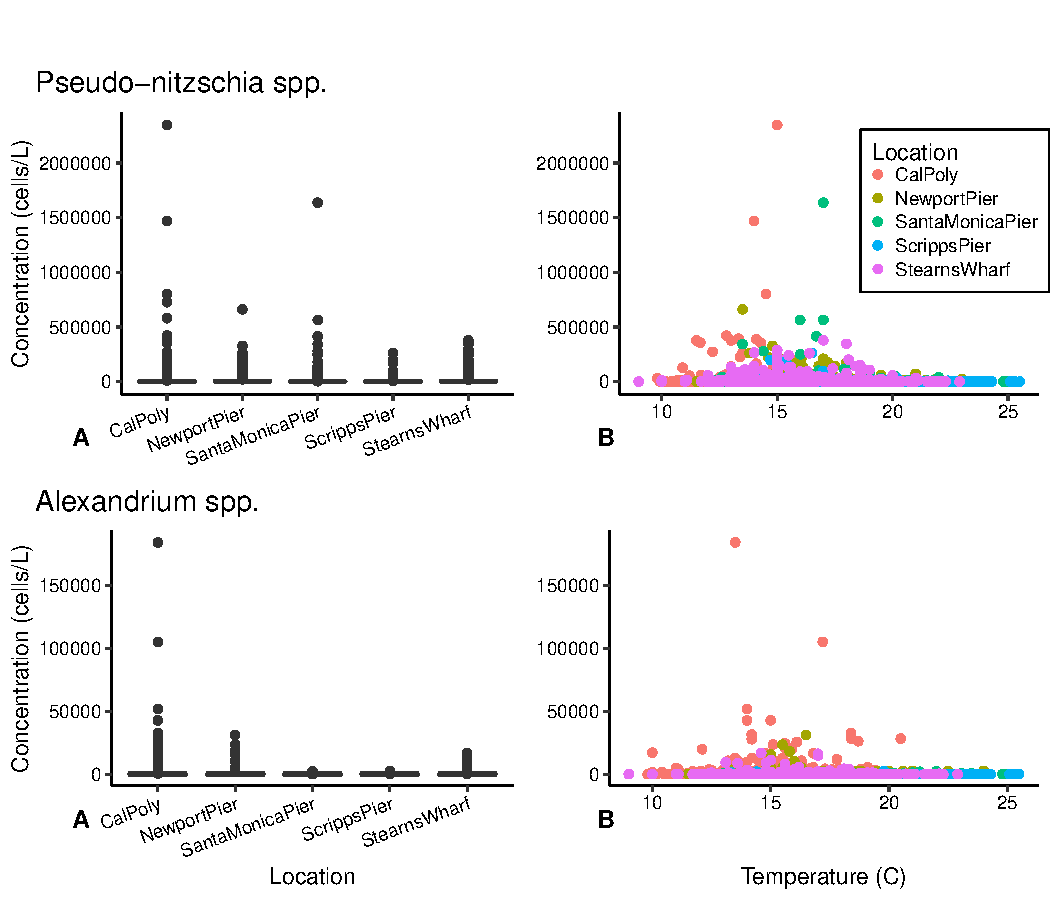
\includegraphics{Habs_Final_Report_files/figure-latex/Exploratory Analysis-1.pdf}

\newpage

Fig. 2 shows the relationship between location and recorded SST. CalPoly
and Stearns Wharf have lower SST's than that of Newport Pier, Santa
Monica Pier, and Scripps Pier. This could be due to the latitudinal
position of each sampling site, as cold water moves southward along the
North American Pacific Coast.

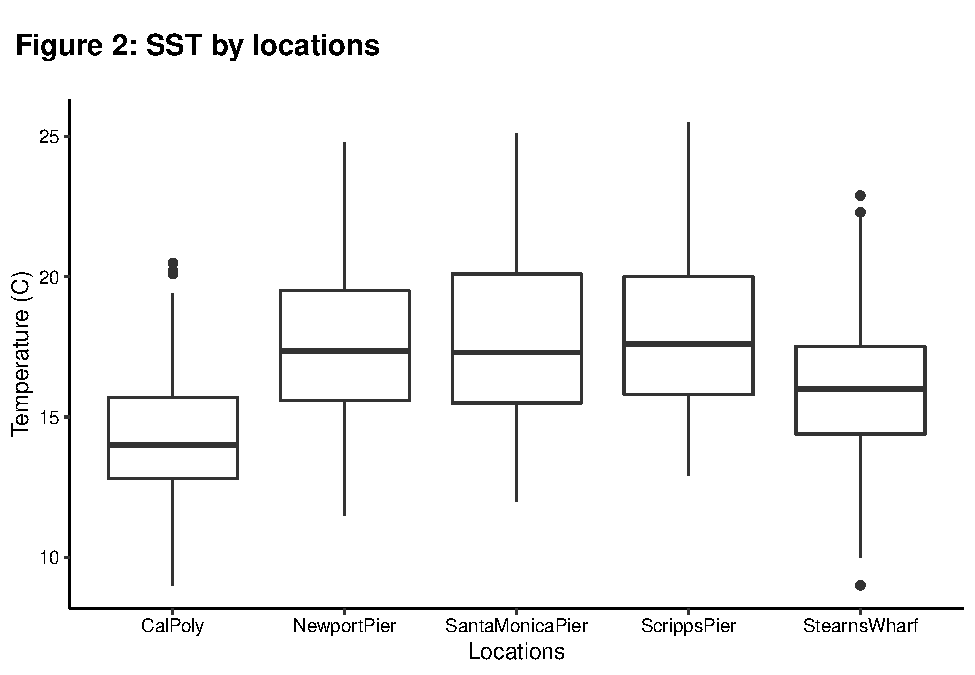
\includegraphics{Habs_Final_Report_files/figure-latex/Exploratory Analysis Part 2 SST-1.pdf}

\newpage

Fig. 3 shows nutrient concentrations over time for each sampling site.
For ammonium (NH4), nitrate (NO3), and silicate (SiO3), there is
indication of seasonality as certain times of the year are associated
with peaks in nutrient concentrations. Ammonium shows an increase
concentration spikes over time at Stearns Wharf while nitrite shows an
increase in concentration spikes at Santa Monica Pier. For phosphate,
most samples have a nutrient concentration of 0 micro-Molar, except for
Santa Monica. For silicates in CalPloy, the data gaps can be observed
pre-2010. Referring to Table 1, the NA values of the dataset are found
in recorded nutrient concentrations and SST.

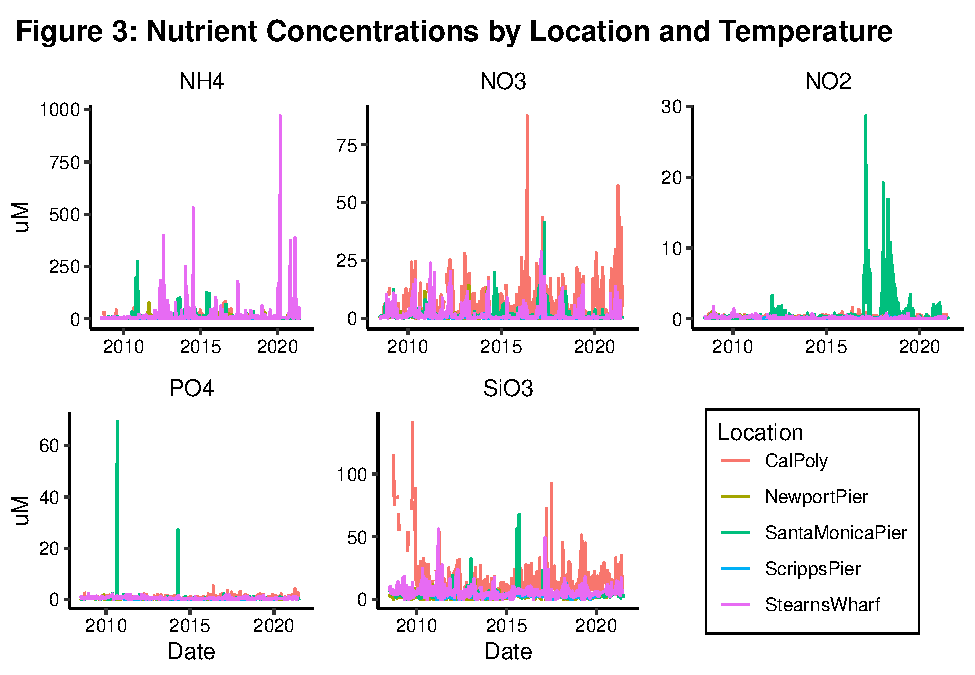
\includegraphics{Habs_Final_Report_files/figure-latex/Exploratory Analysis Part 3-1.pdf}

\newpage

\hypertarget{analysis}{%
\section{Analysis}\label{analysis}}

\hypertarget{time-series}{%
\subsection{Time-Series}\label{time-series}}

Ten time series analyses were performed in this project: five examining
changes in Pseudo-nitzschia concentrations over time at each SCCOOS site
and five examining changes in Alexandrium concentrations over time at
each SCCOOS site. These analyses were conducted by first filtering HAB
data for a specific SCCOOS site and then generating a daily dataset
encompassing that site's date range. The filtered dataset and daily
dataset were then merged using a shared column (date), and a linear
interpolation was used to fill missing HAB data. We felt as though a
linear interpolation was appropriate in this case because missing data
gaps were not large but differences in algal concentrations were
significant. Next, a monthly mean dataset was generated using the
interpolated HAB values; this was the dataset used to establish starting
points, create the time series objects and run the seasonal Mann Kendall
tests. This process was used to create and test each time series object.

\hypertarget{linear-regression-model}{%
\subsection{Linear Regression Model}\label{linear-regression-model}}

To answer question 2, a time-series analysis was conducted to observe
any variables of significance in determining algal concentrations. The
processed data set was split into several groups by location and algal
species. For each group, a linear model was conducted using the same
full model (Algae concentration \textasciitilde{} Ammonium + Nitrate +
Nitrite + Phosphates + Silicates + Temperature + Month of Sample + Year
of Sample) using the ``lm'' R function. Since phosphorous, nitrogen, and
silica compounds are used in algal growth processes, these five nutrient
concentrations were selected for the full models. Temperature, month,
and year were selected to include the relationship between SST and time
on algal growth or decline. Salinity was omitted from this model due to
the higher number of NA's in the dataset. Based on a model's Aikaikie
Information Criterion (AIC), a model would be reduced (using the
backwards step method) to its most parsimonious version. Two tables of
the linear model summaries were created using the tidy() function from
the ``broom'' package''. The variables of each final model, the included
variable's coefficients, and the R-squared value of the final model are
represented in Tables 5 and 6.

\newpage

\hypertarget{results}{%
\section{Results}\label{results}}

\hypertarget{question-1-how-do-concentrations-of-pseudo-nitzschia-and-alexandrium-change-over-time}{%
\subsection{Question 1: How do concentrations of Pseudo-nitzschia and
Alexandrium change over
time?}\label{question-1-how-do-concentrations-of-pseudo-nitzschia-and-alexandrium-change-over-time}}

As delineated by an asterisk in Table 4, the only sites that have
statistically significant trends in HAB concentrations over time are
Newport and San Diego; interestingly, the trends at these locations
(which consist of an upward trend for Pseudo-nitzschia in Newport, a
downward trend for Pseudo-nitzschia in San Diego, and a downward trend
for Alexandrium in both Newport and San Diego) are significant for both
HAB types.

It is important to note that the y-axes are not consistent across the
plot grids in Fig. 4 and Fig. 5, so the slopes of the linear regressions
included in these figures cannot be cross compared. The horizontal line
at 10,000 cells/L in Fig. 4 and at 100 cells/L in Fig. 5 delineate bloom
thresholds for both species.

\begin{longtable}[t]{lll}
\caption{\label{tab:Table 4}Seasonal Mann Kendall Results from Pseudo-nitzschia and Alexandrium Time Series Analyses}\\
\toprule
site & Pseudo-nitzschia p-values & Alexandrium p-values\\
\midrule
Cal Poly & 0.69995 & 0.06883\\
Newport Pier & 0.00045 * & 0.02187 *\\
Santa Monica Pier & 0.24145 & 0.21864\\
Scripps Pier & 0.02199 * & 0.00679 *\\
Stearns Wharf & 0.48946 & 0.11334\\
\bottomrule
\end{longtable}

\newpage

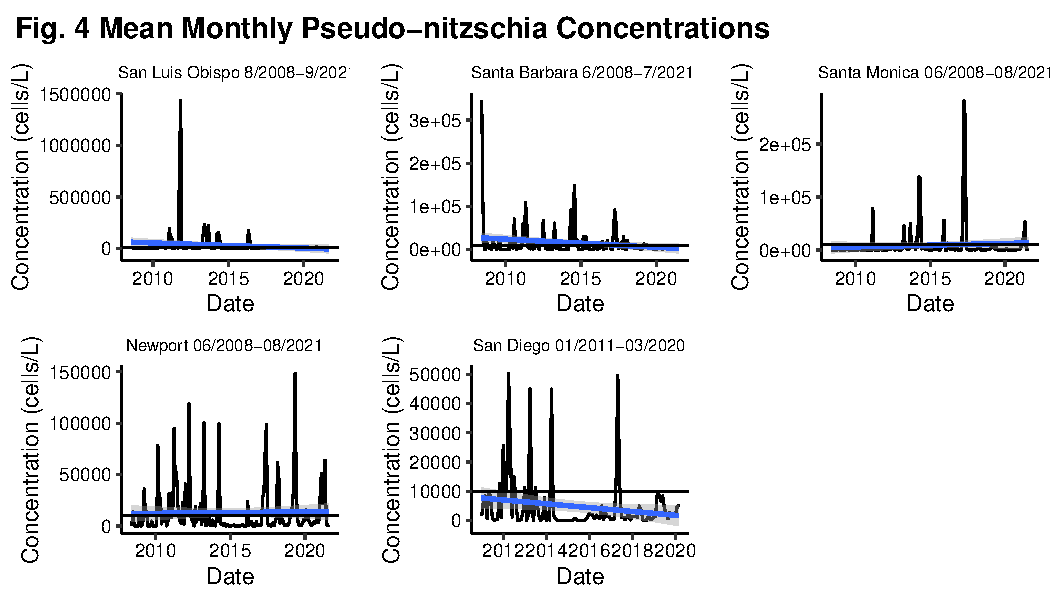
\includegraphics{Habs_Final_Report_files/figure-latex/combining figures-1.pdf}
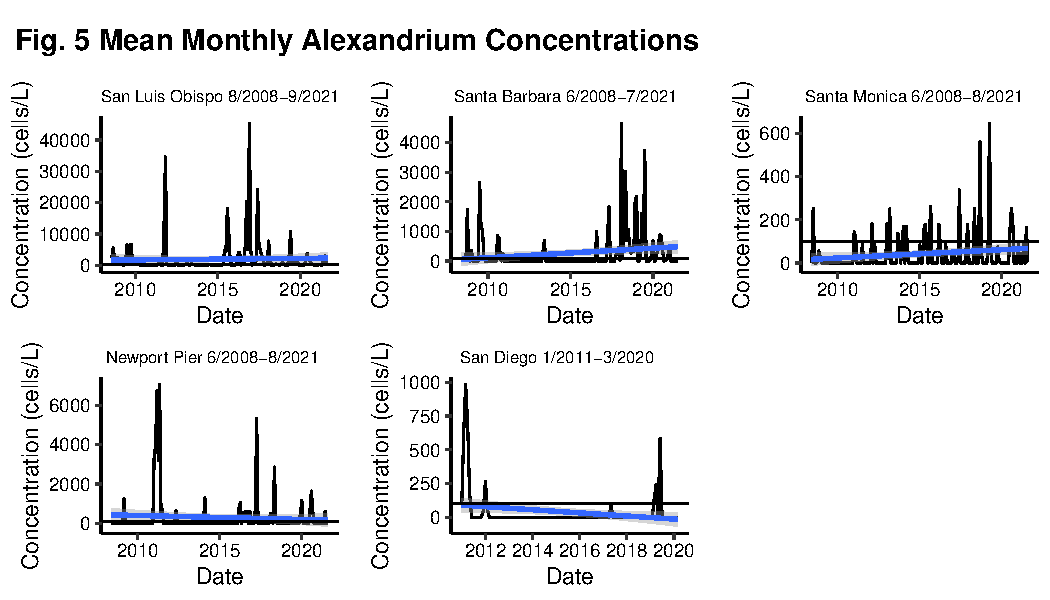
\includegraphics{Habs_Final_Report_files/figure-latex/combining figures-2.pdf}

\newpage

\hypertarget{question-2-which-environmental-variables-help-describe-variation-in-hab-concentrations}{%
\subsection{Question 2: Which environmental variables help describe
variation in HAB
concentrations?}\label{question-2-which-environmental-variables-help-describe-variation-in-hab-concentrations}}

According to Table 5, the concentration of Pseudo-nitzschia are
positively associated with Nitrite concentrations and negatively
associated with Silicate concentrations across sampling locations. The
variables for SST, time, and other nutrients do not show a consistent
pattern across locations. The variable ``Year of Sample'' shows both
positive and negative association with Algae concentration while
Phosphate is included in only one final model for Stearns Wharf. The
R-squared value for most Pseudo-nitzschia models are less than 0.10,
meaning that these models explain less than 10\% of the variance in the
data. The final model for Santa Monica Pier yields a R-squared value of
0.26, explaining 26\% of the variance in algae concentration in Santa
Monica.

For the Alexandrium species group, there is less consistency across
sample locations. No one variable is included in each sampling
location's final model. Phosphate, which is included in the final model
of three locations, shows a positive association with nutrient
concentration. The R-squared values for all final models of Alexandrium
concentrations are below 0.05, explaining less than 5\% of the variance.

\begingroup\fontsize{9}{11}\selectfont

\begin{longtable}[t]{lrrrrrrrr}
\caption{\label{tab:LM Output Tables}Coefficients for Pseudo-nitzschia Linear Models}\\
\toprule
Site & NO3 & NO2 & SiO3 & PO4 & Temp. & Month & Year & R-sq.\\
\midrule
CalPoly & 2547.930 & -55271.86 & -1670.953 & NA & NA & 3397.633 & -10255.709 & 0.0606946\\
NewportPier & 5006.021 & -45449.42 & -2395.457 & NA & -4097.108 & NA & NA & 0.0668576\\
SantaMonicaPier & 14089.827 & 2852.33 & -2203.449 & NA & NA & NA & 1140.451 & 0.2623792\\
ScrippsPier & 2219.378 & NA & -2640.881 & NA & -1501.370 & NA & NA & 0.0608496\\
StearnsWharf & 3023.980 & -45828.06 & -2013.057 & 12277.17 & NA & NA & -1537.447 & 0.0506702\\
\bottomrule
\end{longtable}
\endgroup{}

\begingroup\fontsize{9}{11}\selectfont

\begin{longtable}[t]{lrrrrrr}
\caption{\label{tab:LM Output Tables}Coefficients for Alexandrium Linear Models}\\
\toprule
Site & NO3 & SiO3 & PO4 & Month & Year & R-sq.\\
\midrule
CalPoly & -375.63363 & -52.805512 & 6117.9378 & 330.75946 & NA & 0.0443133\\
NewportPier & NA & NA & 1484.5865 & -62.71097 & NA & 0.0246442\\
SantaMonicaPier & NA & 4.606819 & NA & NA & 3.991525 & 0.0167177\\
ScrippsPier & NA & NA & NA & -9.52388 & -10.159332 & 0.0323822\\
StearnsWharf & -38.01425 & NA & 458.1815 & NA & 46.593697 & 0.0130540\\
\bottomrule
\end{longtable}
\endgroup{}

\newpage

\hypertarget{summary-and-conclusions}{%
\section{Summary and Conclusions}\label{summary-and-conclusions}}

Overall, there was little consistency in HAB trends throughout southern
California; there seems to be a consistent upward trend in Alexandrium
in the more northern study sites but the only statistically significant
trends for Alexandrium are downwards and are further south. Similarly,
the type and strength of trends in Pseudo-nitzschia vary greatly with
p-values ranging from 0.00045 to 0.699.

One interesting similarity between the two HAB types is that the
magnitude of blooms tend to vary greatly across sites. San Luis Obispo
in particular seems to experience blooms that are orders of magnitudes
larger than those experienced by monitoring sites further south; this is
the case for both Pseudo-nitzschia and Alexandrium blooms.

According to the linear models, Pseudo-Nitzschia concentrations are
positively associated with Nitrite and negatively associated with
Silicates. Alexandrium concentrations in select sites are positively
associated with Phosphates. It is important to note that these linear
models do not explain much of the variance. Moving forward, there should
be more review on the interactions of algal species and nutrients. When
algae species grow, they consume the nutrients in the water column and
reduce the overall nutrient concentration. Complications that arise from
this interaction could be mitigated by averaging the nutrient
concentration for the week or month or by converting algae data into
Poisson data; research on the relationship between average nutrient
concentration and average algae concentration would also be helpful
here.

Although the only upward trend of HAB concentrations that we observed
were that of Pseudo-nitzschia concentrations in Newport, this upward
trend has been noted in many species globally over the past 10-15 years
(Lewitus et al.~2012) Consequently, it has become increasingly important
to better understand the dynamics of these destructive and dangerous
phenomena especially as our climate and oceans continue to change.

\newpage

\hypertarget{references}{%
\section{References}\label{references}}

Lewitus, A. J., Horner, R. A., Caron, D. A., Garcia-Mendoza, E., Hickey,
B. M., Hunter, M., Huppert, D. D., Kudela, R. M., Langlois, G. W.,
Largier, J. L., Lessard, E. J., RaLonde, R., Jack Rensel, J. E.,
Strutton, P. G., Trainer, V. L., \& Tweddle, J. F. (2012). Harmful algal
blooms along the North American West Coast Region: History, trends,
causes, and impacts. Harmful Algae, 19, 133--159.
\url{https://doi.org/10.1016/j.hal.2012.06.009}

Moore, S. K., Trainer, V. L., Mantua, N. J., Parker, M. S., Laws, E. A.,
Backer, L. C., \& Fleming, L. E. (2008). Impacts of climate variability
and future climate change on harmful algal blooms and human health.
Environmental Health, 7(Suppl 2).
\url{https://doi.org/10.1186/1476-069x-7-s2-s4}

Smith, J., Connell, P., Evans, R. H., Gellene, A. G., Howard, M. D. A.,
Jones, B. H., Kaveggia, S., Palmer, L., Schnetzer, A., Seegers, B. N.,
Seubert, E. L., Tatters, A. O., \& Caron, D. A. (2018). A decade and a
half of pseudo-nitzschia spp. and domoic acid along the coast of
Southern California. Harmful Algae, 79, 87--104.
\url{https://doi.org/10.1016/j.hal.2018.07.007}

Trainer, V. L., Moore, S. K., Hallegraeff, G., Kudela, R. M., Clement,
A., Mardones, J. I., \& Cochlan, W. P. (2020). Pelagic harmful algal
blooms and climate change: Lessons from nature's experiments with
extremes. Harmful Algae, 91, 101591.
\url{https://doi.org/10.1016/j.hal.2019.03.009}

Zhu, Z., Qu, P., Fu, F., Tennenbaum, N., Tatters, A. O., \& Hutchins, D.
A. (2017). Understanding the blob bloom: Warming increases toxicity and
abundance of the harmful bloom diatom pseudo-nitzschia in California
Coastal Waters. Harmful Algae, 67, 36--43.
\url{https://doi.org/10.1016/j.hal.2017.06.004}

\end{document}
